\chapter{Samples}

\subsection{Periodic AMI operations - Deadline Violation}

\label{sec:AMI}
\noindent\textbf{Description:}\\
The goal of this scenario is to test the utility of the analysis tool in handling AMI calls inside the business logic of component operations. The test consists of two components - a Client and a Server component. The client component is associated with a timer that fires once at every hyperperiod. In the business logic of this timer operation, the Client component makes an AMI call to a provided operation on a remote Server. The client and server are separated by temporal partitions each 50 ms long. Once the client makes an AMI call, the client thread does not block but instead continues with the rest of the timer operation. Meanwhile, the completion of an AMI query of the client side induces a AMI operation on the server side. This operation is run to completion in Partition 2. On completion of the remote method on the server, a callback operation is induced on the client's message queue. When the client is scheduled again, the callback operation is dequeued and completed. The aim of this test is to verify the correctness of the generated CPN and also the correctness of the observed behavior. 

\noindent\textbf{Location:}\\
\texttt{\$F6IAP/f6mde/f6ml/IM/samples/CPNAnalysis\_Samples/ \\ Periodic\_AMI/Deadline\_Violation/}


\noindent\textbf{Expected Results:}\\
The expected results include the following: 
\begin{enumerate}
\item Successfully generate a CPN\_Analysis\_Model and a functions.sml file by using the CPNGenerator interpreter in the modeling tools.
\item The .cpn file is a valid file, i.e., CPN Tools 4 is able to open the colored petri net without any errors.
\item Using the state space tool in CPN Tools, successfully generate a bounded state space - say 10,000 nodes to observe close to 10 hyperperiods of thread activity.
\item Evaluate the deadline monitoring state space query to realize the presence of a deadline violation.
\end{enumerate}

The AMI callback operation on the client side is set with a deadline of 30 ms but the duration of the operation is set to 45 ms to simulate an unexpected delay in completion. On evaluating the deadline monitor in the analysis tool, a violation is observed as soon as the clock of the component node reaches the deadline of the operation. This observation is shown in Figure \ref{fig:Periodic_AMI_DV}.

\begin{figure}[htb]
\centering
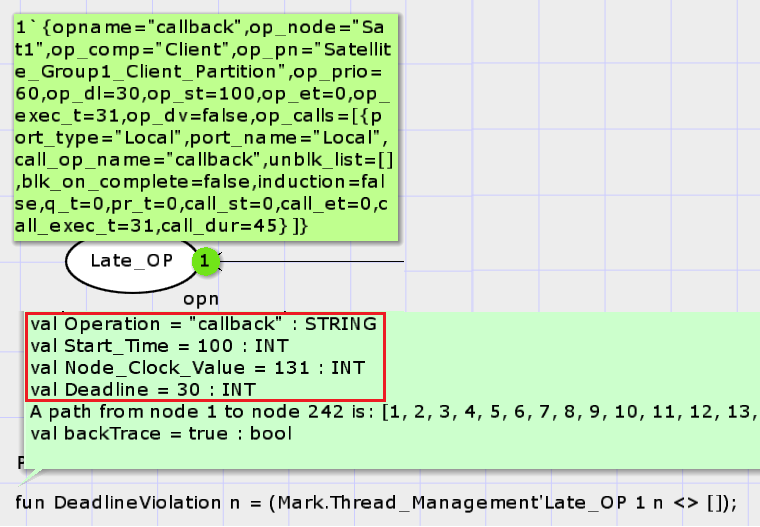
\includegraphics[scale=0.45]{./figs/CPN_Periodic_AMI_DV.png}
\caption{Periodic AMI operations - Deadline Violation}
\label{fig:Periodic_AMI_DV}
\end{figure}

\noindent\textbf{Test Mode:}\\
The mode of testing is manual. Once the colored petri net is generated, the CPN Tools software is used to open the .cpn file, generate a bounded state space and evaluate the generated state space queries to analyze the system.

\noindent\textbf{Prerequisites:}\\
A clean installation of the CPN Tools 4 tool (http://cpntools.org/). This software is required to open, edit, simulate and analyze the generated colored petri nets. 

\subsection{Periodic AMI operations - No Deadline Violation}
\noindent\textbf{Description:}\\
The component assembly of this scenario is identical to \ref{sec:AMI}. However, the duration of the callback operation is reduced to 10 ms and its deadline increased to 60 ms. This motivation for this change is to relax the strictness of the timing specification to allow for timely completion of the scheduled operations. 

\noindent\textbf{Location:}\\
\texttt{\$F6IAP/f6mde/f6ml/IM/samples/CPNAnalysis\_Samples/ \\ Periodic\_AMI/No\_Deadline\_Violation/}


\noindent\textbf{Expected Results:}\\

The expected results include the following: 
\begin{enumerate}
\item Successfully generate a CPN\_Analysis\_Model and a functions.sml file by using the CPNGenerator interpreter in the modeling tools.
\item The .cpn file is a valid file, i.e., CPN Tools 4 is able to open the colored petri net without any errors.
\item Using the state space tool in CPN Tools, successfully generate a bounded state space - say 10,000 nodes to observe close to 10 hyperperiods of thread activity.
\item Evaluate the deadline monitoring state space query to realize the absence of any deadline violations.
\end{enumerate}

The callback operation is enqueued at the same time as in the previous case but only takes 10 ms to complete. Even with the periodicity of the timer triggering new AMI operations, the system remains stable without any deadline violations for the observed duration of time. The state space query produces a negative result in identifying a deadline violation within the observed state space. 

\noindent\textbf{Test Mode:}\\
The mode of testing is manual. Once the colored petri net is generated, the CPN Tools software is used to open the .cpn file, generate a bounded state space and evaluate the generated state space queries to analyze the system.

\noindent\textbf{Prerequisites:}\\
A clean installation of the CPN Tools 4 tool (http://cpntools.org/). This software is required to open, edit, simulate and analyze the generated colored petri nets. 

\subsection{Periodic RMI operations - Deadline Violation}
\label{sec:RMI}

\noindent\textbf{Description:}\\
The goal of this scenario is to test the utility of the analysis tool in handling RMI calls inside the business logic of component operations. The test consists of two components - a Client and a Server component. The client component is associated with a timer that fires once at every hyperperiod. In the business logic of this timer operation, the Client component makes an RMI call to a provided operation on a remote Server. The client and server are separated by temporal partitions each 50 ms long. Once the client makes an RMI call, the client thread starts blocking till the server thread on completes executing the remote method and unblocks the client thread. The deadline of the timer operation is set to 120 ms. The timer fires at time 0 and starts blocking after the RMI call is made. There is no further activity in this partition. At time 50, the server thread is scheduled to execute the RMI operation induced on the server message queue. The server thread executes this operation to completion taking 30 ms, unblocking the client. The client thread however does not get scheduled again till time 100. If the post-processing time for the RMI query and further calculations made on the client exceed the deadline of the timer operation, then a client-side deadline violation is observed.

\noindent\textbf{Location:}\\
\texttt{\$F6IAP/f6mde/f6ml/IM/samples/CPNAnalysis\_Samples/ \\ Periodic\_RMI/Deadline\_Violation/}

\noindent\textbf{Expected Results:}\\

The expected results include the following: 

\begin{enumerate}
\item Successfully generate a CPN\_Analysis\_Model and a functions.sml file by using the CPNGenerator interpreter in the modeling tools.
\item The .cpn file is a valid file, i.e., CPN Tools 4 is able to open the colored petri net without any errors.
\item Using the state space tool in CPN Tools, successfully generate a bounded state space - say 10,000 nodes to observe close to 10 hyperperiods of thread activity.
\item Evaluate the deadline monitoring state space query to realize the presence of a deadline violation.
\end{enumerate}

The RMI call blocks the client thread till time 100 ms. When the client is scheduled again, the amount of work required to complete the client timer operation (26 ms) exceeds the deadline of this operation (120 ms) and so a deadline violation is observed at time 121 ms. This observation can be seen in Figure \ref{fig:Periodic_RMI_DV}

\begin{figure}[htb]
\centering
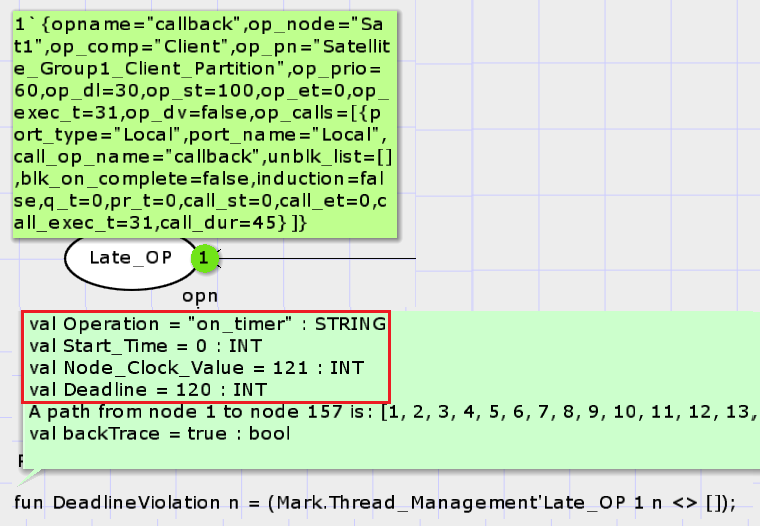
\includegraphics[scale=0.45]{./figs/CPN_Periodic_RMI_DV.png}
\caption{Periodic RMI operations - Deadline Violation}
\label{fig:Periodic_RMI_DV}
\end{figure}

\noindent\textbf{Test Mode:}\\
The mode of testing is manual. Once the colored petri net is generated, the CPN Tools software is used to open the .cpn file, generate a bounded state space and evaluate the generated state space queries to analyze the system.

\noindent\textbf{Prerequisites:}\\
A clean installation of the CPN Tools 4 tool (http://cpntools.org/). This software is required to open, edit, simulate and analyze the generated colored petri nets. 

\subsection{Periodic RMI operations - No Deadline Violation}

\noindent\textbf{Description:}\\
The component assembly of this scenario is identical to \ref{sec:RMI}. However, the deadline of the client timer operation is relaxed by 10 ms to provide for a timely completion. 

\noindent\textbf{Location:}\\
\texttt{\$F6IAP/f6mde/f6ml/IM/samples/CPNAnalysis\_Samples/ \\ Periodic\_RMI/No\_Deadline\_Violation/}

\noindent\textbf{Expected Results:}\\
The expected results include the following: 
\begin{enumerate}
\item Successfully generate a CPN\_Analysis\_Model and a functions.sml file by using the CPNGenerator interpreter in the modeling tools.
\item The .cpn file is a valid file, i.e., CPN Tools 4 is able to open the colored petri net without any errors.
\item Using the state space tool in CPN Tools, successfully generate a bounded state space - say 10,000 nodes to observe close to 10 hyperperiods of thread activity.
\item Evaluate the deadline monitoring state space query to realize the absence of any deadline violations.
\end{enumerate}
The client timer operation completes at time 126 ms which is 4 ms short of its deadline and so no deadline violations are observed and the system is stable. 

\noindent\textbf{Test Mode:}\\
The mode of testing is manual. Once the colored petri net is generated, the CPN Tools software is used to open the .cpn file, generate a bounded state space and evaluate the generated state space queries to analyze the system.

\noindent\textbf{Prerequisites:}\\
A clean installation of the CPN Tools 4 tool (http://cpntools.org/). This software is required to open, edit, simulate and analyze the generated colored petri nets. 

\subsection{Trajectory Planning Application - Deadline Violation due to RMI blocking delay}
\label{sec:TPA_S1}

\noindent\textbf{Description:}\\
The component assembly for this application consists of two components: A \emph{Sensor} component and a \emph{Trajectory Planner} component. The Sensor component periodically publishes on a trigger topic, notifying the Trajectory Planner of the existence of new sensor data. Once the notification is received, the Trajectory Planner makes an RMI call to retrieve the data structure of sensor values. Using the updated sensor values, the Trajectory Planner calculates a new trajectory for the satellite. 

Figure \ref{fig:TPA_TD} shows the partition schedule and temporal behavior considered. The sensor component operates on partition 1, and the trajectory planner operates on partition 2. Both partitions have a duration of 20 ms and a period of 40 ms. The sensor component is associated with a periodic timer that fires every 80 ms. When this timer expires, the sensor component publishes on a notification topic. Accounting for network latencies, the analysis assumes that this task does not take more than 8 ms. Once the notification is sent out, the sensor component becomes passive. With DDS push semantics, this notification manifests itself as a DDS operation on the trajectory planner's message queue. When partition 2 becomes active, the trajectory planner component receives the notification is has subscribed to, after which it makes an RMI call to the sensor component to obtain the updated sensor values. After the RMI call is made, this component blocks for the remainder of the partition. When the sensor component is scheduled again, it services the RMI request and sends out the RMI response, effectively unblocking the trajectory planner. Once the new sensor data is retrieved, the trajectory planner calculates a new trajectory for the satellite node.

While modeling this application using the modeling tools, BusinessLogic atoms are connected to appropriate ports in each Component's Implementation and the timing specification for the different operations are correctly written. Once the Business Logic of the component operations are correctly configured, the CPNGenerator Interpreter is used to generate a CPN Analysis Model. The interpreter generates two files: a CPN\_Analysis\_Model.cpn and a functions.sml file.  

The .cpn file is an analyzable colored petri net. Using CPN Tools 4, simulation and state space-based analysis are carried out on the generated net. This particular scenario shows the utility of the analysis tool in identifying missed deadlines in component operations. In this case, if the Trajectory Planner component thread blocks on the RMI call for longer than its configured deadline, the analysis tool identifies the missed deadline and provides a backtrace of state space nodes that lead to a deadline violation. 

\begin{figure}
        \centering
        \begin{subfigure}[b]{0.5\textwidth}
                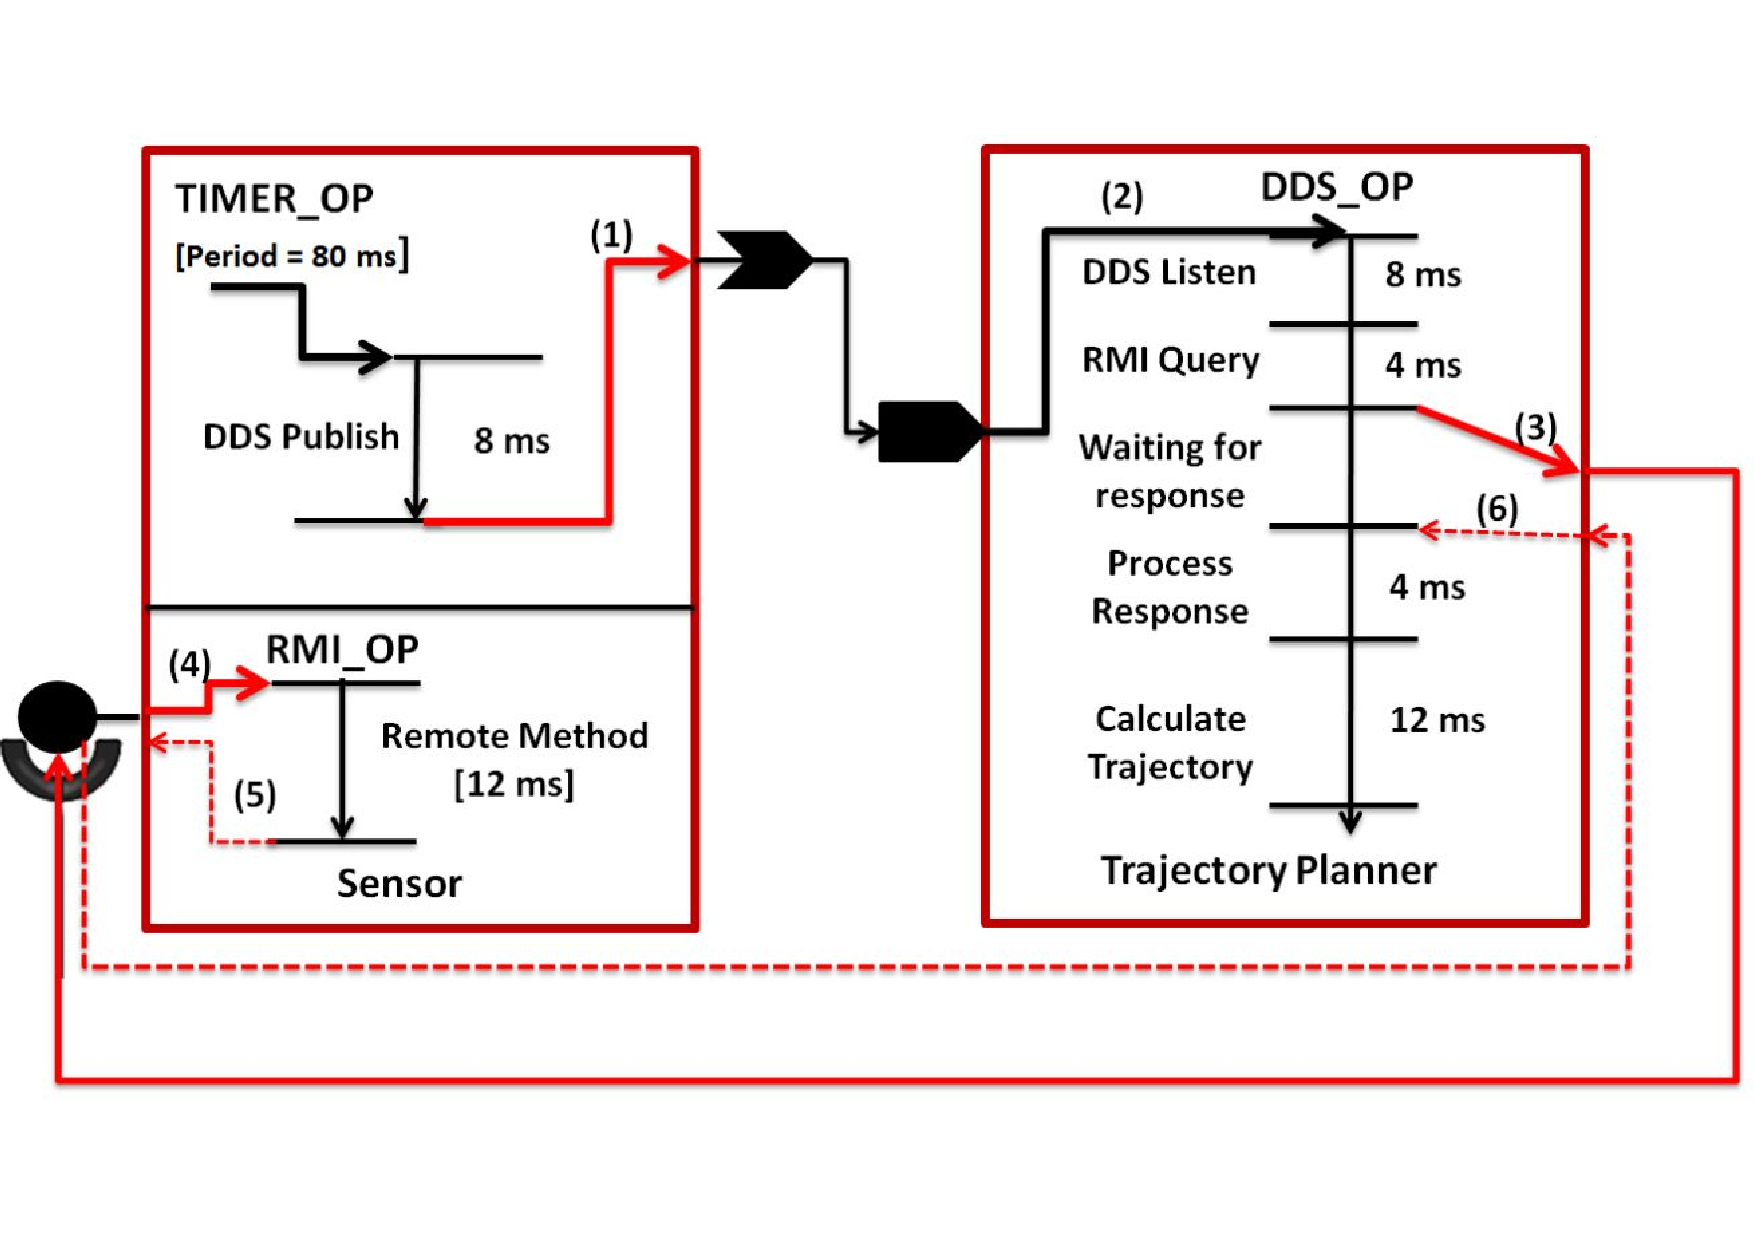
\includegraphics[width=\textwidth]{./figs/CPN_TPA}
                \caption{Component Assembly}
                \label{fig:CA}
        \end{subfigure}%
        \begin{subfigure}[b]{0.5\textwidth}
                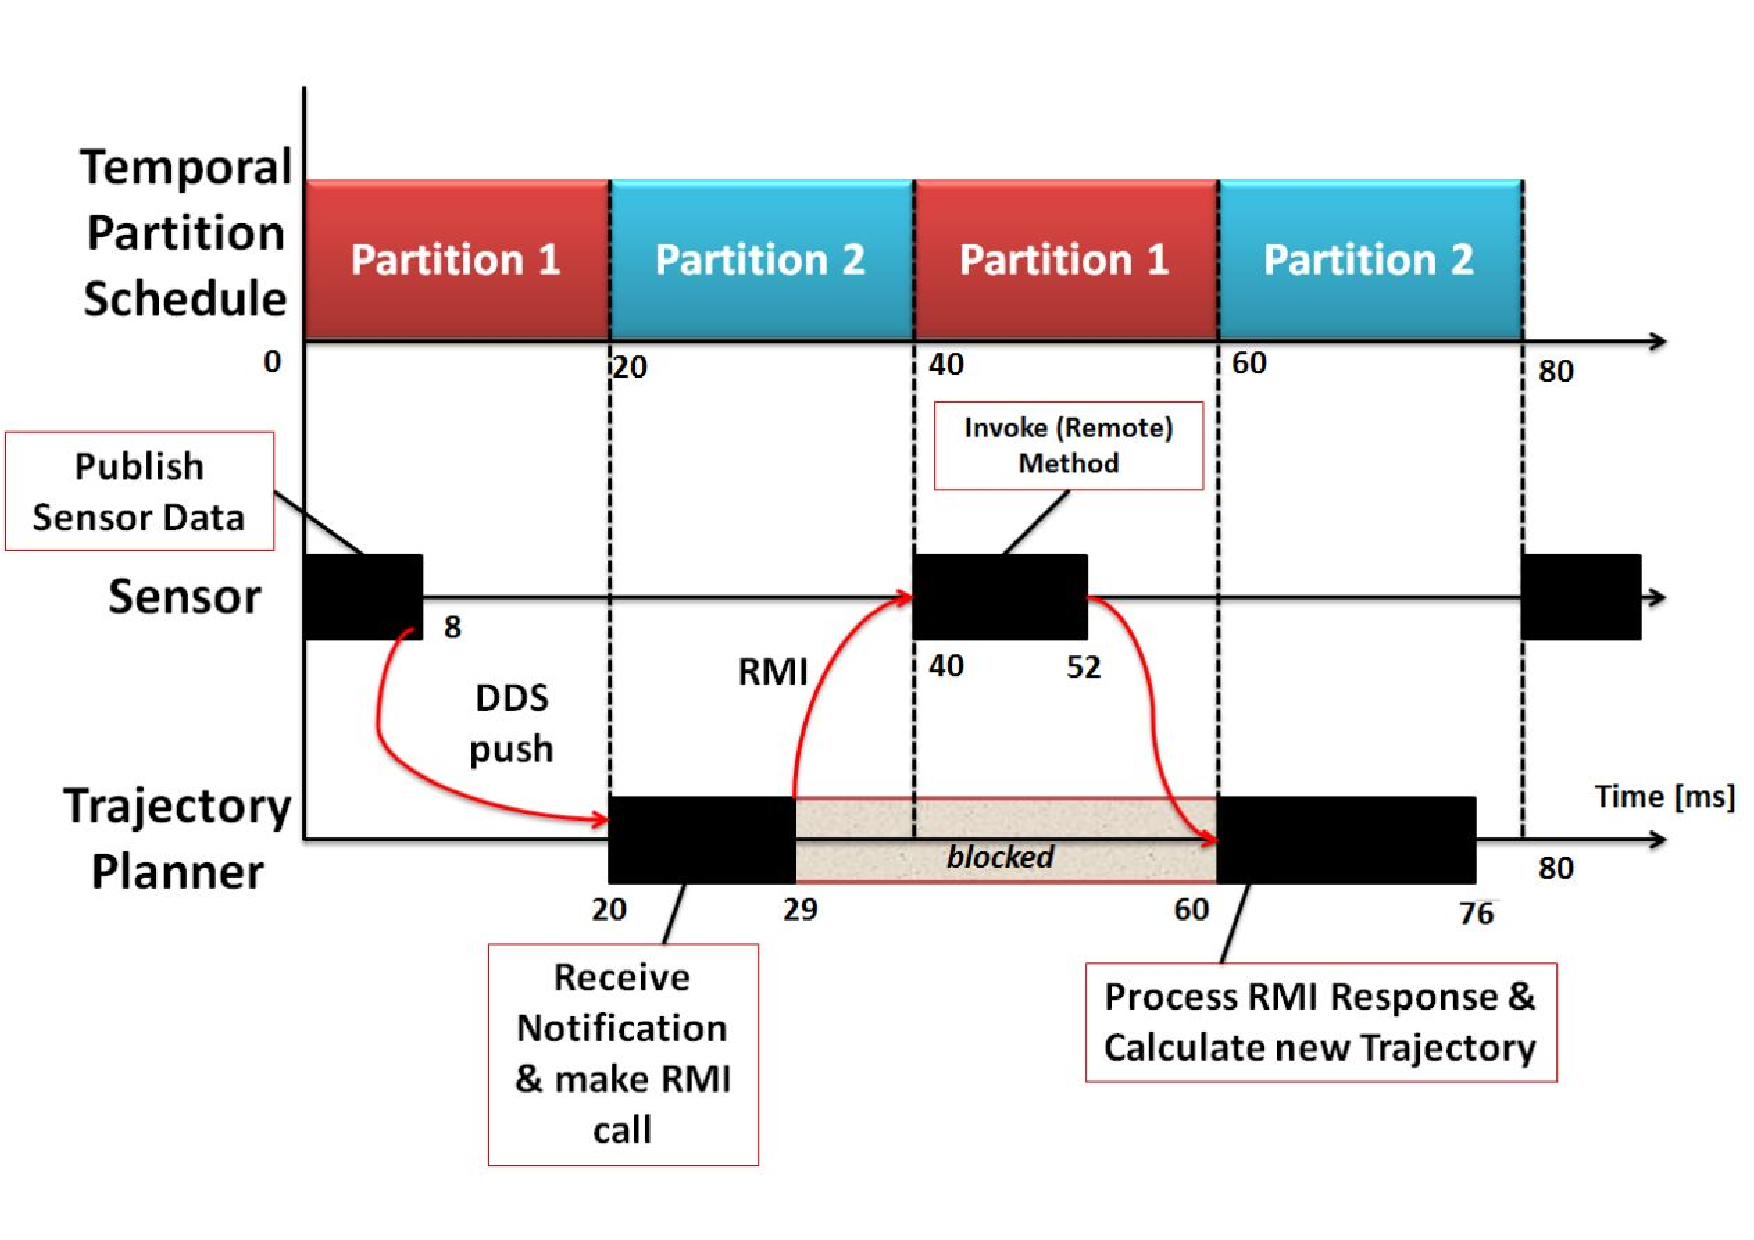
\includegraphics[width=\textwidth]{./figs/CPN_TPA_TD}
                \caption{Timing Diagram}
                \label{fig:TPA_TD}
        \end{subfigure}
        \caption{Trajectory Planning Application}\label{fig:TPA}
\end{figure}

\noindent\textbf{Location:}\\
\texttt{\$F6IAP/f6mde/f6ml/IM/samples/CPNAnalysis\_Samples/ \\ Trajectory\_Planning\_Application}
   \texttt{/Scenario\_1\_RMI\_Blocking\_Delay/}

\noindent\textbf{Expected Results:}\\

The expected results include the following: 
\begin{enumerate}
\item Successfully generate a CPN\_Analysis\_Model and a functions.sml file by using the CPNGenerator interpreter in the modeling tools.
\item The .cpn file is a valid file, i.e., CPN Tools 4 is able to open the colored petri net without any errors.
\item Using the state space tool in CPN Tools, successfully generate a bounded state space - say 10,000 nodes to observe close to 10 hyperperiods of thread activity.
\item Evaluate the deadline monitoring state space query to realize the presence of a deadline violation.
\end{enumerate}
The deadline for the DDS push subscribe operation of the Trajectory Planner is set to 50 ms. This operation starts at a time stamp of 20 ms (at the start of Partition 2). However this operation does not complete till time stamp 76 as shown in \ref{fig:TPA_TD}. This missed deadline is observed as the result of evaluating the state space query.

\noindent\textbf{Test Mode:}\\
The mode of testing is manual. Once the colored petri net is generated, the CPN Tools software is used to open the .cpn file, generate a bounded state space and evaluate the generated state space queries to analyze the system.

\noindent\textbf{Prerequisites:}\\
A clean installation of the CPN Tools 4 tool (http://cpntools.org/). This software is required to open, edit, simulate and analyze the generated colored petri nets. 


\subsection{Trajectory Planning Application - Deadline Violation due to high frequency of timer expiry}

\noindent\textbf{Description:}\\
The component assembly of this scenario is identical to the setup in \ref{sec:TPA_S1}. The frequency of the timer that triggers the Sensor to publish notifications is increased by 8 times. Instead of a period of 80 ms, the timer now has a period of 10 ms. Each timer leads to an infrastructural operation in the Sensor's message queue. Each of these operations has a strict deadline. If the timer expiry is not handled in time, the operations that are enqueued in message queue every 10 ms miss the configured deadline eventually. The analysis aims to identify a deadline violations that are caused by such frequent timer operation requests. 

\noindent\textbf{Location:}\\
\texttt{\$F6IAP/f6mde/f6ml/IM/samples/CPNAnalysis\_Samples/ \\ Trajectory\_Planning\_Application}
\texttt{/Scenario\_2\_Timer\_Expiry\_Frequency/}

\noindent\textbf{Expected Results:}\\

The expected results include the following: 
\begin{enumerate}
\item Successfully generate a CPN\_Analysis\_Model and a functions.sml file by using the CPNGenerator interpreter in the modeling tools.
\item The .cpn file is a valid file, i.e., CPN Tools 4 is able to open the colored petri net without any errors.
\item Using the state space tool in CPN Tools, successfully generate a bounded state space - say 10,000 nodes to observe close to 10 hyperperiods of thread activity.
\item Evaluate the deadline monitoring state space query to realize the presence of a deadline violation.
\end{enumerate}

The deadline of each timer operation is set to 10 ms. However, after each timer operation, the Trajectory Planner receives a notification and makes an RMI call to the Sensor, just as in \ref{sec:TPA_S1}. This RMI call manifests as a facet operation on the Sensor. As shown in \ref{fig:TPA_TD}, the Sensor executes the RMI operation at time 40. Therefore, the Sensor is unable to service the intermediate timer expiry at time 40 ms. The expected result of state space analysis is that the tool identifies a missed deadline at time 51 ms. The timer that expired at 40 ms does not get serviced before its deadline, 10 ms. 

\noindent\textbf{Test Mode:}\\
The mode of testing is manual. Once the colored petri net is generated, the CPN Tools software is used to open the .cpn file, generate a bounded state space and evaluate the generated state space queries to analyze the system.

\noindent\textbf{Prerequisites:}\\
A clean installation of the CPN Tools 4 tool (http://cpntools.org/). This software is required to open, edit, simulate and analyze the generated colored petri nets. 

\subsection{Trajectory Planning Application - Deadline Violation due to publish operations in a loop}

\noindent\textbf{Description:}\\
The goal of this scenario is to test the utility of the analysis tool in handling control loops in the business logic. The CPNGenerator interpreter identifies loops in the business logic of component operations and transforms this nature into appropriate colored petri net tokens that can be used for analysis. The component assembly of this test is similar to \ref{sec:TPA_S1}. The business logic of the timer operation is changed such that the DDS publish step is written inside a control loop. 

\noindent\textbf{Location:}\\
\texttt{\$F6IAP/f6mde/f6ml/IM/samples/CPNAnalysis\_Samples/ \\ Trajectory\_Planning\_Application/}
\texttt{Scenario\_3\_Publishing\_in\_a\_loop/}

\noindent\textbf{Expected Results:}\\

The expected results include the following: 
\begin{enumerate}
\item Successfully generate a CPN\_Analysis\_Model and a functions.sml file by using the CPNGenerator interpreter in the modeling tools.
\item The .cpn file is a valid file, i.e., CPN Tools 4 is able to open the colored petri net without any errors.
\item Using the state space tool in CPN Tools, successfully generate a bounded state space - say 10,000 nodes to observe close to 10 hyperperiods of thread activity.
\item Evaluate the deadline monitoring state space query to realize the presence of a deadline violation.
\end{enumerate}

Each operation publishes on the Notification topic thrice inside a control loop. The deadline is this operation is 30 ms but the operation should only take 24 ms. However, there is an unconditional partition switch at time 20 ms after which the Sensor component is scheduled again only at time 40. Therefore even the first timer operation completes only at time 44 ms, leading to a missed deadline. 

\noindent\textbf{Test Mode:}\\
The mode of testing is manual. Once the colored petri net is generated, the CPN Tools software is used to open the .cpn file, generate a bounded state space and evaluate the generated state space queries to analyze the system.

\noindent\textbf{Prerequisites:}\\
A clean installation of the CPN Tools 4 tool (http://cpntools.org/). This software is required to open, edit, simulate and analyze the generated colored petri nets. 

\subsection{Trajectory Planning Application - Multinode scenario}

\noindent\textbf{Description:}\\
The goal of this scenario is to test the utility of the analysis tool in efficiently handling multi-node deployments. The component assembly is identical to \ref{sec:TPA_S1} but the software bundle consists of copies of this application deployed on multiple nodes. 

\noindent\textbf{Location:}\\
\texttt{\$F6IAP/f6mde/f6ml/IM/samples/CPNAnalysis\_Samples/ \\ Trajectory\_Planning\_Application/}
\texttt{Scenario\_4\_Multinode/}

\noindent\textbf{Expected Results:}\\
The deadlines of all operations are set to large enough values that none of the operations miss deadlines. The CPNGenerator generates a valid CPN model with correct tokens for a multi-node scenario. This includes (1) multiple clock and schedule tokens, one for each node, (2) multiple instances of the Sensor and Trajectory Planner threads, one for each node, (3) multiple instances of component message queues for each thread, one for each node, and (4) a timer token for each Sensor component instance in the bundle. Generating a state space of around 50,000 nodes should be sufficient to observe 10 hyperperiods of thread activity on each node. 

\noindent\textbf{Test Mode:}\\
The mode of testing is manual. Once the colored petri net is generated, the CPN Tools software is used to open the .cpn file, generate a bounded state space and evaluate the generated state space queries to analyze the system.

\noindent\textbf{Prerequisites:}\\
A clean installation of the CPN Tools 4 tool (http://cpntools.org/). This software is required to open, edit, simulate and analyze the generated colored petri nets. 

\subsection{Two-way RMI call - Deadlock}
\label{sec:Two_Way_RMI}

\noindent\textbf{Description:}\\
The goal of this scenario is to test the utility of the analysis tool in identifying system deadlocks. The component assembly (Figure \ref{CPN_RMI_DLK}) consists of two components - a client and a server. When a timer expires on the client component, the client thread makes an RMI call to the server component and starts blocking. When the server component services the requested operation, the server makes an RMI call to an exposed operation on the client. The server starts blocking after dispatching this query. Since both the client and server are blocked on each other, the system reaches a state of deadlock.

\noindent\textbf{Location:}\\
\texttt{\$F6IAP/f6mde/f6ml/IM/samples/CPNAnalysis\_Samples/ \\ TwoWay\_RMI\_Deadlock/}

\begin{figure}[htb]
\centering
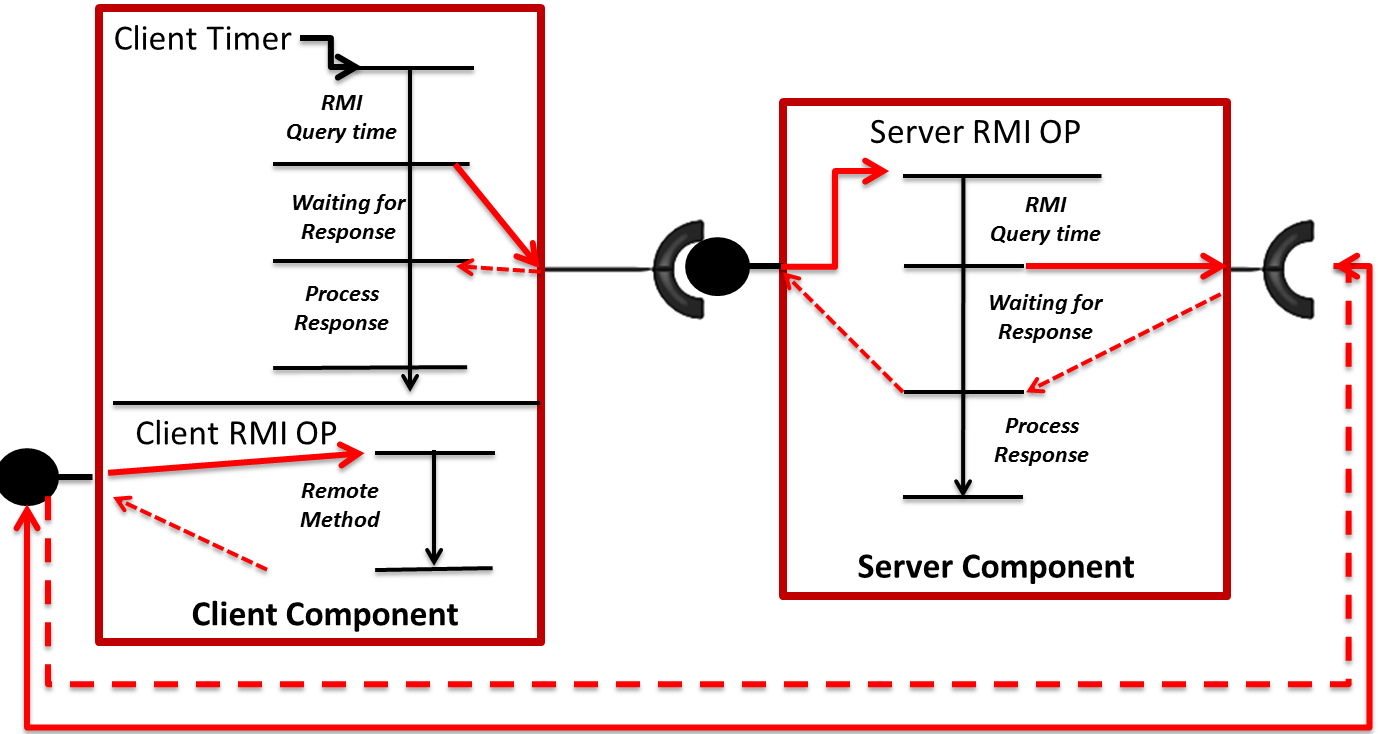
\includegraphics[scale=0.30]{./figs/CPN_RMI_DLK.png}
\caption{Two-Way RMI Deadlock}
\label{fig:CPN_RMI_DLK}
\end{figure}

\noindent\textbf{Expected Results:}\\

The expected results include the following: 
\begin{enumerate}
\item Successfully generate a CPN\_Analysis\_Model and a functions.sml file by using the CPNGenerator interpreter in the modeling tools.
\item The .cpn file is a valid file, i.e., CPN Tools 4 is able to open the colored petri net without any errors.
\item Using the state space tool in CPN Tools, successfully generate a bounded state space - say 10,000 nodes to observe close to 10 hyperperiods of thread activity.
\end{enumerate}

At the end of the first hyperperiod, the client is done dispatching an RMI query to the server and the server is done dispatching an RMI query to the client. Both component threads are blocked on each other and the system reaches a state of deadlock.

\noindent\textbf{Test Mode:}\\
The mode of testing is manual. Once the colored petri net is generated, the CPN Tools software is used to open the .cpn file. Since there is only one possible thread execution order to this scenario, the CPN Tools simulation tool can be used to progress simulation by 100-200 steps. Once the first hyperperiod of activity is complete, the place \emph{BT} indicating the list of blocked thread tokens should hold two tokens - (1) a token representing the client thread blocked on the server and (2) a token representing the server thread blocked on the client. At this point, the system is in the state of deadlock and only the \emph{Progress\_Time} transition should be enabled. 

\noindent\textbf{Prerequisites:}\\
A clean installation of the CPN Tools 4 tool (http://cpntools.org/). This software is required to open, edit, simulate and analyze the generated colored petri nets. 